\documentclass[11pt,a4paper]{article}

\usepackage[T1]{fontenc}
\usepackage[utf8]{inputenc}
\usepackage{times}
\usepackage[a4paper,top=0.75in,bottom=0.75in,left=0.65in,right=0.65in]{geometry}
\usepackage{amsmath,amssymb}
\usepackage{graphicx}
\usepackage{booktabs}
\usepackage{enumitem}
\usepackage{titlesec}
\usepackage{hyperref}
\usepackage{setspace}
\usepackage{parskip}
\usepackage{tikz}
\usetikzlibrary{arrows.meta,positioning,shapes.geometric}

\setstretch{1.0}
\setlength{\parskip}{0.4em}

\titleformat{\section}
{\normalsize\bfseries}
{\thesection.}{0.5em}{}
\titlespacing*{\section}{0pt}{0.6em}{0.2em}

\titleformat{\subsection}
{\normalsize\bfseries}
{\thesubsection.}{0.5em}{}

\setlist[itemize]{topsep=2pt,itemsep=1pt,leftmargin=1.5em}
\hypersetup{hidelinks}

\begin{document}

% SOURCE: https://aqora.io/challenges/global-industry-challenge-2026/tracks/gic-2026-qBraid-MITRE-JonesTrading :: challenge year and phase
\begin{center}
{\large \textbf{Quantum Reservoir Computing for Forecasting Equity
Volatility Regime Transitions}}

{\small Team QTyche}

\textbf{\small Global Industry Challenge 2026 $\cdot$ Phase 3
Submission $\cdot$ Track A}
\end{center}

\section{Introduction and contribution}

Volatility regimes influence risk limits, hedging and execution, while
transitions are precisely the periods in which persistence assumptions can
fail. We therefore separate two related tasks: classifying the low/medium/high
regime of forward realised variance, including transition discrimination, and
forecasting its continuous magnitude. Reservoir computing is attractive
because a fixed nonlinear dynamical system can expose a rich feature map while
training only a classical readout \cite{jaeger2001echo,fujii2017harnessing}.

We evaluate rather than assume the value of a compact quantum reservoir. The
study combines leakage-safe, validation-only architecture selection; complete
classical controls; controlled finite-shot/noise analysis; formal paired
statistics; a genuine-MNIST benchmark; and independent qBraid clean-room
reproduction. All quantum states are produced by exact classical simulation.
The aim is a transparent account of when the selected QRC is competitive, not
a claim of quantum advantage.

\section{Data, targets and evaluation protocol}

% SOURCE: data/processed/public_market/data_manifest.json :: snapshot_id, source_symbols, canonical_start_date, canonical_end_date
The frozen public snapshot \texttt{yahoo\_chart\_20100101\_20251231\_v1}
contains adjusted daily observations for SPY and QQQ and levels for VIX from
4 January 2010 through 31 December 2025. Sixteen causal inputs cover returns,
trailing realised and Parkinson volatility, volume/range, VIX, QQQ and weekday
families. Preprocessing statistics are fitted on training data only.

% SOURCE: data/processed/public_market/data_manifest.json :: split_details
Chronological splits contain 2,744 training observations
(2 February 2010--23 December 2020), 748 validation observations
(4 January 2021--21 December 2023), and 497 test observations
(2 January 2024--23 December 2025). Five trading days are purged at each
boundary, and no sample is shuffled.

% SOURCE: data/processed/public_market/data_manifest.json :: target_definition, forward_horizon_days
For daily log return \(r_t\), the target is the annualised forward five-day
realised variance
\[
 y_t=\frac{252}{5}\sum_{k=1}^{5} r_{t+k}^{\,2}.
\]
% SOURCE: data/processed/public_market/data_manifest.json :: regime_thresholds
Low, medium and high labels use only the training-target 0.33 and 0.66
quantiles (0.00663709 and 0.01954608). A transition is a future label different
from the current trailing-volatility label. Classification uses macro-F1,
balanced accuracy and transition PR-AUC; continuous forecasts use QLIKE, RMSE,
MAE and correlation. QLIKE is emphasised because it is robust for variance
forecast evaluation \cite{patton2011volatility}.

\section{Final QRC and classical controls}

% SOURCE: configs/reproduction/final_financial_qrc.yaml :: model, simulator, readout
The final financial reservoir has two qubits, two virtual nodes and the
\texttt{reset\_each\_input} policy. Each market observation starts from the
configured initial density matrix; within that observation, the input qubit is
partially traced and re-injected at each virtual substep, so state is retained
across the two substeps but never across market dates. A fixed seeded Gaussian
projection \(b_v^\top x_t\) sets
\(\theta_{t,v}=0.5b_v^\top x_t\), encoded as
\(R_y(\theta_{t,v})|0\rangle\) on the input qubit.

% SOURCE: configs/reproduction/final_financial_qrc.yaml :: reservoir
Each substep evolves for half of total time \(\tau=1\) under the fixed random
transverse-field Ising Hamiltonian
\[
 H=\sum_{(i,j)\in E}J_{ij}Z_iZ_j+\sum_i h_iX_i,
\]
where \(E\) is the unique edge of the two-qubit ring, seeded
\(J_{ij}\!\sim U[-1,1]\) and \(h_i\!\sim U[0.5,1.5]\).
Expectations of \(Z_0,Z_1,Z_0Z_1\) at each virtual node give six features.
This temporal multiplexing increases observable density without increasing
qubit count; it does not create cross-date memory.

% SOURCE: configs/reproduction/final_financial_qrc.yaml :: architecture.n_qubits, architecture.virtual_nodes, architecture.observables
\begin{center}
\begin{minipage}{\linewidth}
\centering
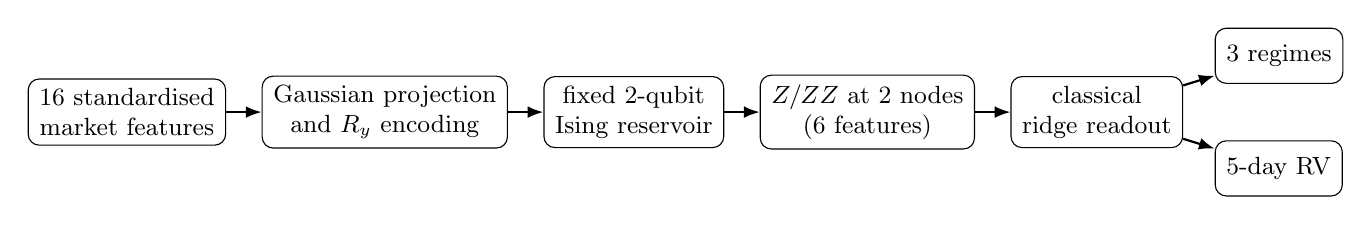
\begin{tikzpicture}[
  node distance=4.5mm,
  box/.style={draw,rounded corners,align=center,minimum height=7mm,
              inner xsep=4pt,font=\small},
  arrow/.style={-{Latex[length=2mm]},thick}
]
\node[box] (x) {16 standardised\\market features};
\node[box,right=of x] (enc) {Gaussian projection\\and \(R_y\) encoding};
\node[box,right=of enc] (qrc) {fixed 2-qubit\\Ising reservoir};
\node[box,right=of qrc] (obs) {\(Z/ZZ\) at 2 nodes\\(6 features)};
\node[box,right=of obs] (read) {classical\\ridge readout};
\node[box,above right=-1mm and 4mm of read] (cls) {3 regimes};
\node[box,below right=-1mm and 4mm of read] (rv) {5-day RV};
\draw[arrow] (x) -- (enc);
\draw[arrow] (enc) -- (qrc);
\draw[arrow] (qrc) -- (obs);
\draw[arrow] (obs) -- (read);
\draw[arrow] (read) -- (cls);
\draw[arrow] (read) -- (rv);
\end{tikzpicture}
\par\smallskip
{\small\textbf{Figure 1:} Final financial pipeline. The fixed exact-simulation reservoir creates
six nonlinear observables per date; only the two classical readouts are fitted.
Architecture and ridge choices use validation data, never test outcomes.\par}
\end{minipage}
\end{center}

% SOURCE: configs/reproduction/final_financial_qrc.yaml :: ridge_grid, reservoir_seeds
Unpenalised-intercept ridge readouts predict three one-hot regime indicators
(then apply a stable softmax) and log realised variance (then exponentiate).
Candidate ridge penalties \(10^{-5},10^{-3},10^{-1},1\) are selected on
validation macro-F1 or QLIKE. Results average the frozen reservoir seeds 2026,
2027 and 2028; probabilities and forecasts are not ensembled.

% SOURCE: paper_assets/tables/publication_table_2_financial_benchmark.json :: rows[].model
% SOURCE: configs/reproduction/garch_baseline.yaml :: model
Strong controls test whether the QRC adds value rather than supply easy
comparisons: majority and regime-persistence classifiers, logistic regression,
realised-variance persistence, an Echo State Network (ESN), and a Gaussian
GARCH(1,1) \cite{bollerslev1986generalized}. Every comparable model uses the
same dates and target definitions.

\section{Financial results and statistical analysis}

% SOURCE: paper_assets/tables/publication_table_2_financial_benchmark.json :: rows
% Generated by prepare_assets.py from the frozen Stage 2C JSON.
% SOURCE: paper_assets/tables/publication_table_2_financial_benchmark.json :: rows
\begin{center}
\begin{minipage}{\linewidth}
\centering
{\small\textbf{Table 1:} Frozen 2024--2025 financial test results. Higher is better except for QLIKE, RMSE and MAE. QRC is mean across three reservoir seeds; the full-precision population standard deviations are retained in the source manifest. Bold marks the best listed point estimate per metric. GARCH has no transition score.\par}
\smallskip
\begin{minipage}[t]{0.515\textwidth}
\centering\small
\begin{tabular}{@{}lrrr@{}}
\toprule
Classifier & Macro-F1 & Bal.\ acc. & Trans.\ PR-AUC \\
\midrule
Majority classifier & 0.151 & 0.333 & 0.506 \\
Regime persistence & 0.485 & 0.485 & 0.511 \\
Logistic regression & \textbf{0.526} & \textbf{0.529} & \textbf{0.683} \\
ESN & 0.446 & 0.478 & 0.645 \\
GARCH(1,1) & 0.373 & 0.442 & \textemdash \\
QRC mean & 0.454 & 0.491 & 0.640 \\
\bottomrule
\end{tabular}
\end{minipage}\hfill
\begin{minipage}[t]{0.455\textwidth}
\centering\small
\begin{tabular}{@{}lrrrr@{}}
\toprule
Forecaster & QLIKE & RMSE & MAE & Corr. \\
\midrule
RV persistence & -2.397 & 0.0866 & 0.0255 & 0.335 \\
ESN & -2.865 & \textbf{0.0662} & \textbf{0.0183} & 0.532 \\
GARCH(1,1) & \textbf{-2.895} & 0.0740 & 0.0233 & 0.356 \\
QRC mean & -2.814 & 0.0894 & 0.0216 & \textbf{0.543} \\
\bottomrule
\end{tabular}
\end{minipage}
\end{minipage}
\end{center}


The QRC is competitive in selected dimensions but does not dominate.
% SOURCE: paper_assets/final_results_manifest.json :: financial.test
Logistic regression leads regime classification (macro-F1 0.526 versus QRC
0.454); GARCH leads QLIKE (\(-2.895\) versus \(-2.814\)); and ESN leads RMSE
(0.0662 versus 0.0894) and MAE (0.0183 versus 0.0216). QRC attains the highest
listed forecast correlation (0.543) and a transition PR-AUC of 0.640, but
point-estimate leadership on one metric is not systematic superiority.

% SOURCE: paper_assets/figures/publication_figure_2_financial_comparison.pdf
% SOURCE: paper_assets/figure_captions.md :: caption 2
\begin{center}
\begin{minipage}{\linewidth}
\centering
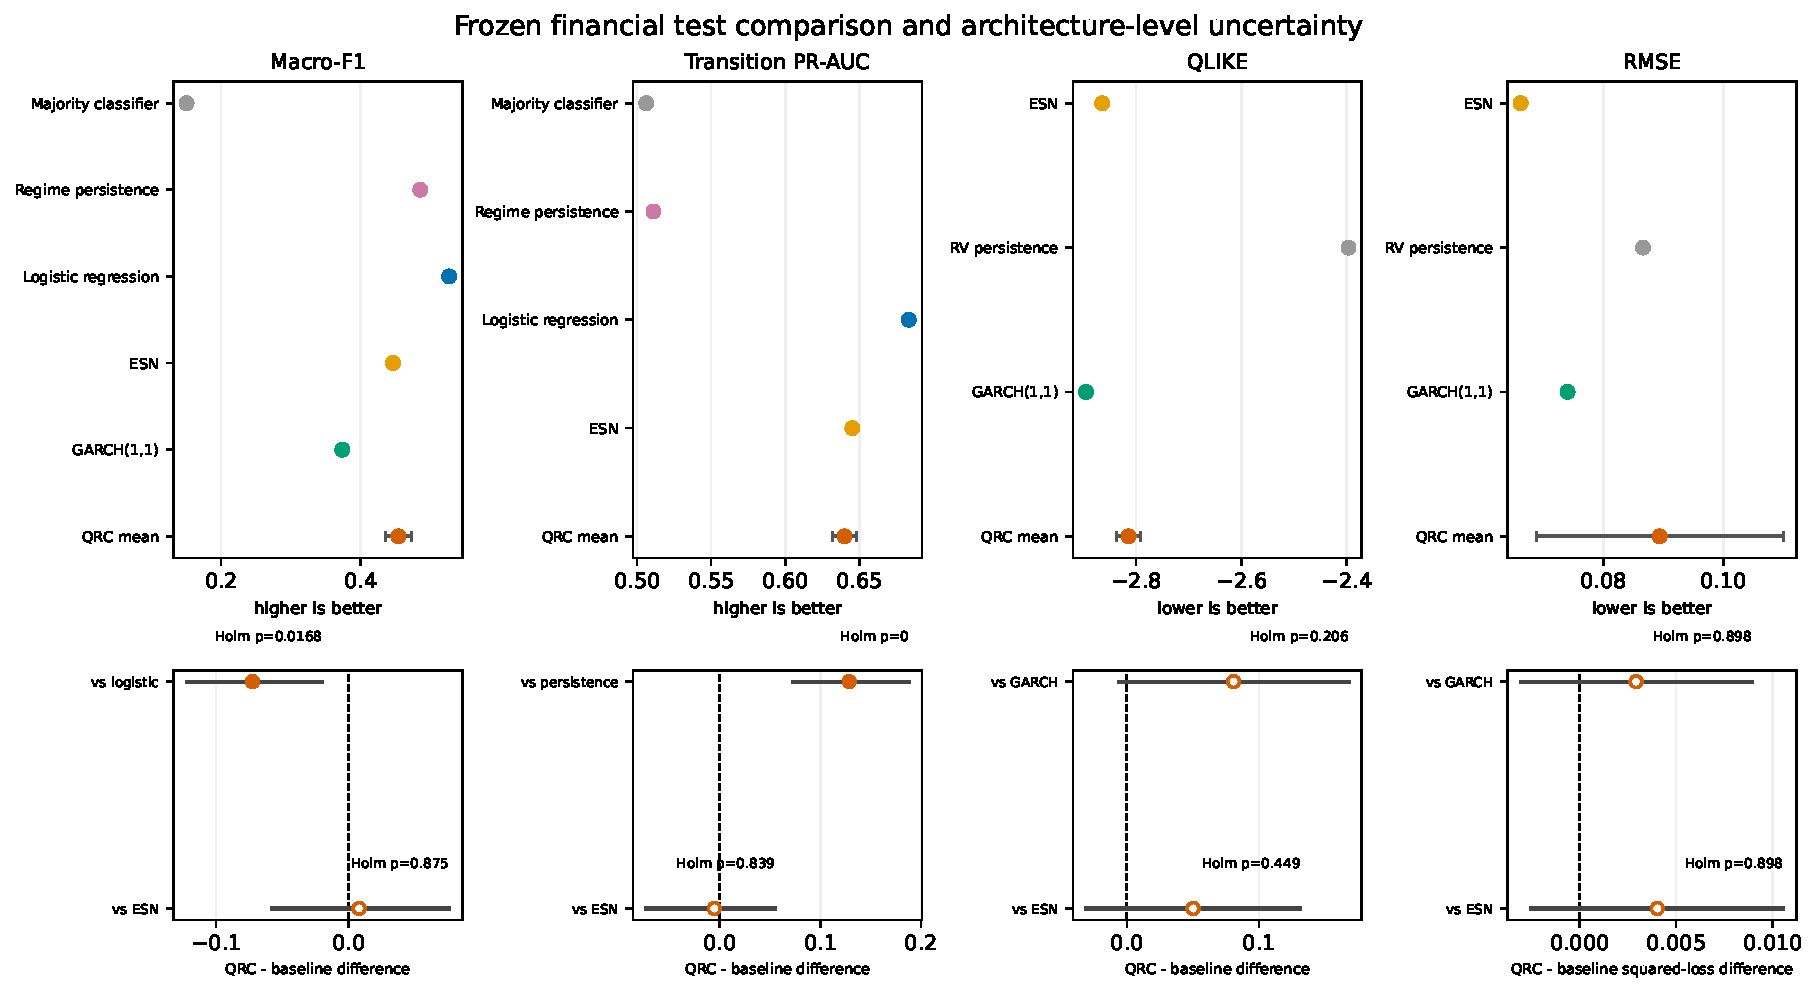
\includegraphics[width=0.97\linewidth]{figures/financial_comparison.pdf}
\par\smallskip
{\small\textbf{Figure 2:} Frozen financial test estimates and selected architecture-level
95\% intervals for QRC-minus-baseline differences. Filled markers denote
Holm-adjusted support and hollow markers do not. QRC statistics average paired
per-seed differences, not prediction ensembles. Logistic leads macro-F1,
GARCH leads QLIKE and ESN leads RMSE.\par}
\end{minipage}
\end{center}

% SOURCE: paper_assets/final_results_manifest.json :: financial.inference
Formal tests use 10,000 paired replicates. Financial losses use a
Diebold--Mariano-style test \cite{diebold1995comparing} with Bartlett
Newey--West HAC lag 4 \cite{newey1987simple}, a five-step finite-sample
correction and circular-block intervals; classification metrics are recomputed
within paired circular blocks. Holm correction is applied within predeclared
metric families. QRC-minus-logistic macro-F1 is \(-0.0726\)
(95\% interval \([-0.1223,-0.0202]\), adjusted \(p=0.0168\)).
QRC exceeds regime persistence in transition PR-AUC by 0.1289
(95\% interval \([0.0733,0.1880]\), adjusted resampling \(p=0\) at the
10,000-replicate resolution).
No QRC-versus-ESN financial classification metric, nor any financial
regression architecture comparison, is Holm-significant. Failure to reject is
not evidence of equivalence.

Post-freeze diagnostics preserve training-derived regime and tail thresholds.
They examine calibration, transition types, rolling errors and high-volatility
tails without refitting. These checks expose limited probability calibration,
small tail samples and a near-singular feature matrix for one seed; they are
descriptive and do not alter the Stage 2A inference or model selection.

\section{Genuine MNIST, robustness and portability}

% SOURCE: configs/qrc_mnist_benchmark.yaml :: dataset, split, model
The independent MNIST benchmark uses checksum-pinned official IDX files
\cite{lecun1998gradient} and balanced, disjoint splits of 6,000 training,
1,000 validation and 1,000 official-test images. Each \(28\times28\) image is
scaled by 255 and compressed row-wise into five fixed column-band means. The
five-qubit, two-virtual-node ring reservoir resets between images and carries
state only across the 28 rows of one image. Five \(Z\) and five ring-edge
\(ZZ\) observables per virtual node are reduced by seven fixed temporal summaries to
140 image features. Training-only standardisation and validation macro-F1
select the multinomial-logistic readout.

% SOURCE: paper_assets/tables/publication_table_3_mnist_benchmark.json :: rows[section=Model comparison]
% Generated by prepare_assets.py from the frozen Stage 2C JSON.
% SOURCE: paper_assets/tables/publication_table_3_mnist_benchmark.json :: rows[section=Model comparison]
\begin{center}
\begin{minipage}{\linewidth}
\centering\small
\textbf{Table 2:} Genuine-MNIST test results. QRC values are mean $\pm$ population standard deviation across the three frozen reservoir seeds; baselines are single deterministic fits.\par
\smallskip
\begin{tabular}{@{}lrrrr@{}}
\toprule
Model & Accuracy & Macro-F1 & Bal.\ acc. & Macro AUC \\
\midrule
Flattened logistic & 0.889 & 0.888 & 0.889 & 0.987 \\
Size-controlled ESN & \textbf{0.934} & \textbf{0.934} & \textbf{0.934} & \textbf{0.995} \\
Exact QRC mean & 0.874 $\pm$ 0.005 & 0.874 $\pm$ 0.005 & 0.874 $\pm$ 0.005 & 0.987 $\pm$ 0.001 \\
\bottomrule
\end{tabular}
\end{minipage}
\end{center}


% SOURCE: paper_assets/final_results_manifest.json :: mnist.test, mnist.robustness
Frozen exact QRC mean accuracy is \(0.874\pm0.005\), compared with 0.889 for
flattened logistic regression and 0.934 for the size-controlled ESN. The ESN
is Holm-significantly higher on all four reported metrics; QRC versus logistic
is not Holm-significant. For seed 2026, accuracy falls from 0.871 analytically
to 0.504 with 2,048 sampled measurements, 0.492 with added depolarising
probability 0.01, and 0.485 with measurement-flip probability 0.02. These
controlled simulations show finite-shot/noise sensitivity, not physical-device
performance \cite{chen2020temporal}.

% SOURCE: paper_assets/figures/publication_figure_4_mnist_benchmark.pdf
% SOURCE: paper_assets/figure_captions.md :: caption 4
\begin{center}
\begin{minipage}{\linewidth}
\centering
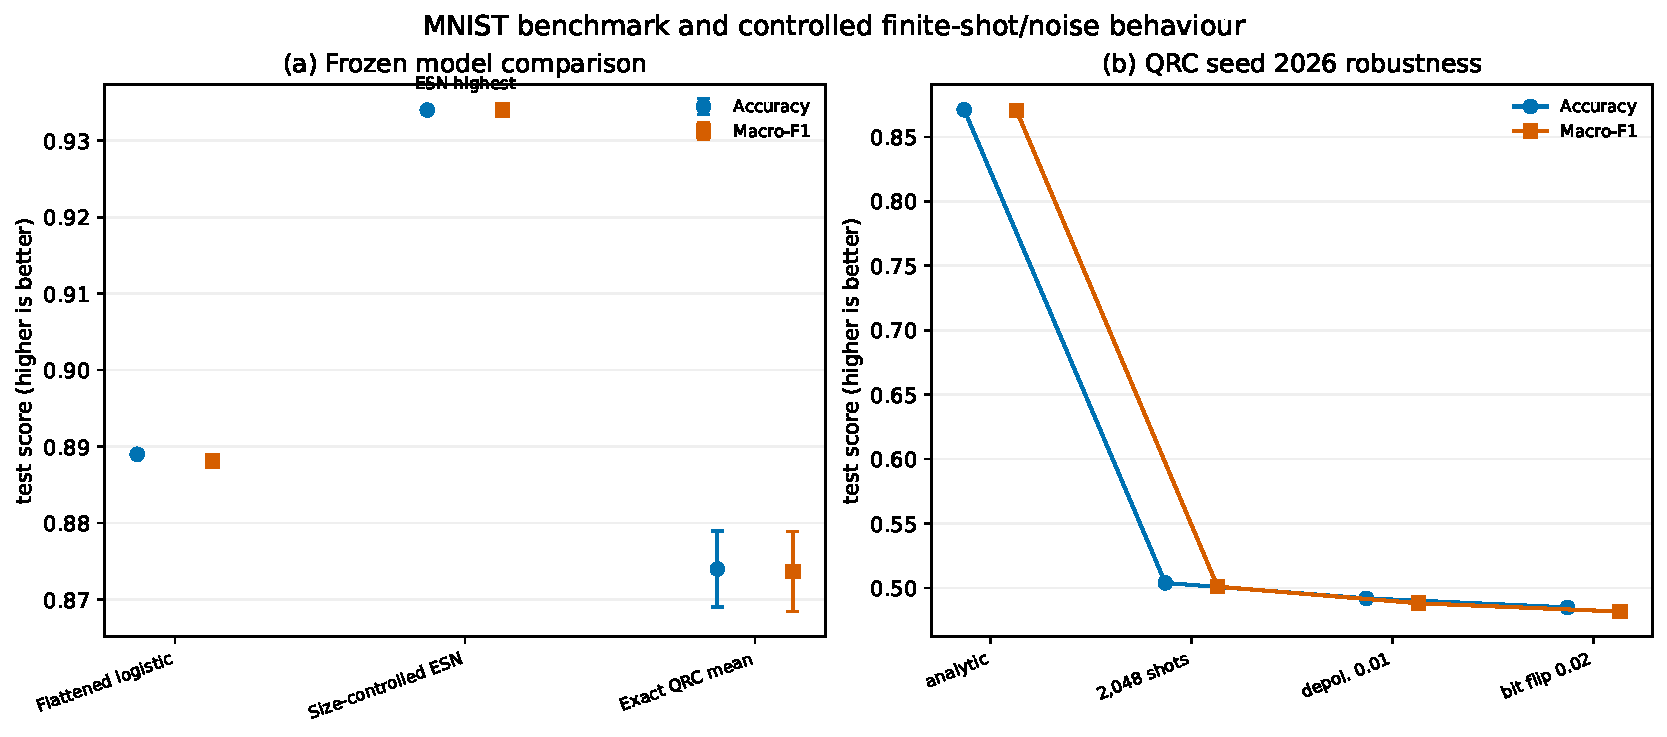
\includegraphics[width=0.92\linewidth]{figures/mnist_benchmark.pdf}
\par\smallskip
{\small\textbf{Figure 3:} Genuine-MNIST test comparison and controlled robustness. Exact QRC
bars show mean and population variation across three seeds; finite-shot/noise
rows use frozen seed 2026. The 2,048-shot, depolarising and measurement-flip
conditions are classical simulations, not hardware-calibrated experiments.\par}
\end{minipage}
\end{center}

% SOURCE: configs/reproduction/mnist_exact_portability_reference.json :: root_cause, publication_value_policy, summary
\newpage
The qBraid e0l4 clean-room run (Python 3.12.3, Linux/x86\_64) verified identical
official files, partitions, preprocessing, architecture, seeds and protocol,
yet reproduced QRC mean accuracy 0.875 rather than the frozen macOS/ARM 0.874.
Across 3,000 test seed--image evaluations, 14 predictions changed, for a net
gain of three correct predictions. Reservoir features first differ only at
floating-point last bits (at most \(6.44\times10^{-15}\)) and, with either
frozen readout, change no decisions.
The divergence enters when platform-sensitive BLAS/L-BFGS convergence selects
nearby multinomial-readout iterates on ill-conditioned designs. The accepted
contract checks features, coefficients, scores, predictions and confusion
matrices; rankings and scientific conclusions are unchanged.

\section{Limitations, reproducibility and conclusion}

% SOURCE: paper_assets/limitations_factsheet.md :: all bullets
The main limitations are classical exponential-cost state simulation, only
three reservoir seeds, overlapping forward targets, small high-volatility
tails, information loss in the MNIST band compression, and sharp degradation
under the frozen finite-shot conditions. The controlled noise channels are not
hardware calibrated, and no physical QPU was executed.

% SOURCE: configs/phase3_reproduction.yaml :: environment, tasks
% SOURCE: configs/reproduction/processed_data_semantic_reference.json :: contract
% SOURCE: configs/reproduction/garch_portability_reference.json :: comparison_contract
Reproduction uses a checksum-pinned Python environment and a resumable
orchestrator. Immutable raw inputs remain SHA-256 exact. Generated financial
tables require exact rows, dates, splits, labels, missingness and thresholds;
finite decimals are canonically committed at 10 significant digits, whose
maximum relative quantisation width is \(10^{-9}\). A separately gated GARCH
portability contract accepts only equivalent optimiser endpoints and forecast
paths; the observed metric drift was below \(9\times10^{-8}\), inside a
GARCH-only \(2.5\times10^{-7}\) metric envelope, with unchanged threshold
crossings, rankings and displayed values. The qBraid full workflow also
regenerated statistical, diagnostic and publication artefacts.

The compact QRC demonstrates useful nonlinear expressivity and competitive
performance in selected settings, but it establishes neither quantum advantage
nor systematic superiority over strong classical models. Its principal value
here is a falsifiable, reproducible assessment of where a small
exact-simulation QRC is competitive, where classical methods remain stronger,
and how numerical portability affects hybrid quantum--classical workflows.

\begingroup
\small
\setlength{\parskip}{0pt}
\bibliographystyle{unsrt}
\bibliography{references}
\endgroup

\end{document}
